\anonsection{Задание 10}
\anonsubsection{Формулировка задания}

Произвести фильтрацию одномерного процесса Орнштейна--Уленбека:
\begin{enumerate}
	\item Используя генератор белого шума, добавить случайную ошибку с 
     известной дисперсией к реализации процесса Орнштейна--Уленбека.
	
	\item При помощи одномерного фильтра Калмана оценить траекторию 
     процесса по зашумленному сигналу. Параметры процесса и белого шума 
     считать известными.
	
	\item Рассмотреть случай, когда шум
	
	\begin{itemize}
		\item Является гауссовским.
		
		\item Имеет распределение Коши.
		
	\end{itemize}
	
\end{enumerate}


\anonsubsection{Добавление случайной ошибки}

\begin{definition}
	Дискретным белым шумом называется последовательность \( \varepsilon_1, 
     \ dots, \varepsilon_n, \dots \) независимых одинаково распределённых 
     случайных величин.
\end{definition}

Рассмотрим соотношение 
\[
x_{k+1}=f(x_k)+\omega(k),
\]
где \( \omega(k) \)~---~случайная помеха, \( x_k \), \( \omega(k) \) 
 независимы, \( f(x_k)=\mathbb{E}(x_{k+1}|x_k) \). Пусть рассматривается 
 марковский процесс, тогда совместная плотность по всем моментам времени
\[
p(x_k,\ldots,x_0)=p(x_k|x_{k-1},\ldots,x_0)\cdot p(x_{k-1}|x_{k-2}, \dots, 
 x_0) \cdot \ldots \cdot p(x_1|x_0) \cdot p(x_0)=
\]
\[
=\lbrace\text{марковский процесс}\rbrace=p(x_k|x_{k-1})\cdot p(x_{k-1} 
| x_{k-2}) \cdot \ldots \cdot p(x_1|x_0)\cdot p(x_0).
\]
Обратим внимание, что в случае, когда шум имеет распределение Коши, 
 фильтрацию провести не получится. Это связанно с тем, что распределение 
 Коши не имеет математического ожидания.  Далее будем рассматривать случай, 
 когда шум является гауссовским (\( \omega(k) \) и \( x_k \) имеют 
 гауссовское распределение).


\anonsubsection{Фильтр Калмана}

Рассмотрим линейное стохастическое уравнение
\[
x_{k+1}=A_kx_k+\omega_k.
\]

Поскольку случайные величины гауссовские, то для их полного описания 
 достаточно знать их первые и вторые моменты.

Пусть имеется следующая система:
\begin{equation} \label{kalman_syst}
\left\lbrace
\begin{array}{rcl}
x_{k+1}&=&A_kx_k+w_k,\\
y_{k+1}&=&C_{k+1}x_{k+1}+v_{k+1},
\end{array}
\right.
\end{equation}
причём \( x_0, w_0,\ldots, w_{N-1},v_0,\ldots,v_{n-1} \) независимы в 
 совокупности. \( Y_{N-1}=(y_0,\ldots,y_{N-1})^T \)~---~все наблюдения, 
 а \( X_{N-1}=(x_0,\ldots,x_{N-1}) \)~---~исходный процесс, его надо найти. 
 Для этого воспользуемся так называемым фильтром Калмана, а точнее, его 
 схемой "<шагаем--мерим">, общий вид которой совпадает с 
 системой~(\ref{kalman_syst}). 

Обозначим \( \mathbb{E} x_0 = \overline{x}_0, \mathbb{D}x_0 = S, 
 \mathbb{E} w_k = \mathbb{E}v_k = 0, \mathbb{D} w_k = M_k, \mathbb{D}v_k = 
 N_k>0 \). Фильтр Калмана для схемы "<шагаем--мерим"> имеет вид:
\[
\left\lbrace
\begin{array}{rcl}
\hat{x}_{k+1|k}&=&A_k\hat{x}_{k|k},\\
\hat{x}_{k+1|k+1}&=&\hat{x}_{k+1|k}+R_{k+1|k}C^T_{k+1}(C_{k+1}R_{k+1|k} 
 C^T_{k+1}+N_{k+1})^{-1}(y_{k+1}-C_{k+1}\hat{x}_{k+1|k}),\\
R_{k+1|k}&=&A_kR_{k|k}A_k^T+M_k,\\
R_{k+1|k+1}&=&R_{k+1|k}-R_{k+1|k}C^T_{k+1}(C_{k+1}R_{k+1|k}C_{k+1}^T+
 N_{k+1})^{-1}C_{k+1}R_{k+1|k},\\
\hat{x}_{0|0}&=&\overline{x}_0,\\
R_{0|0}&=&S.
\end{array}
\right.
\]

В нашей задаче \( x_{k} \)~---~процесс Орнштейна--Уленбека с параметрами 
 \( \sigma_W \) и \( \lambda \), \( y_{k+1}=x_{k+1}+v_{k+1} \), где 
 \( v \)~---~белый шум. Пусть \( \sigma_n^2 \)~---~его дисперсия. Тогда 
 получаем, что \( N_k=\sigma_n^2 \), а \( C_k=1 \). Осталось найти 
 \( A_k \) и \( M_k \). Будем считать, что \( t_{i+1}-t_i=\Delta t \) 
 независимо от \( i \). Так как мы рассматриваем одномерный процесс 
 Орнштейна--Уленбека, то \( A_k,C_k \) являются скалярами, и от их 
 транспонирования ничего не меняется. Обозначим \( \mathbb{D}x_k=V_k \). 
 С одной стороны, имеем
\[
\mathbb{D}x_{k+1}=A_k^2\mathbb{D}x_{k}+\mathbb{D}w_k=A_k^2V_k+M_k,
\]
\[
\text{cov}(x_{k+1},x_k)=\mathbb{E}(x_{k+1}x_k)-\mathbb{E}x_{k+1}\mathbb{E}
 x_k=\mathbb{E}(A_kx_k^2+w_{k+1}x_{k})-A_k(\mathbb{E}x_k)^2=
\]
\[
=\lbrace\mathbb{E}w_{k+1}=0,w_{k+1}\text{ и }x_k\text{ независимы}\rbrace = 
 A_k\left(\mathbb{E}x_k^2-(\mathbb{E}x_k)^2\right)=A_k\mathbb{D}x_k=A_kV_k.
\]

С другой стороны, так как ковариационная функция процесса Орнштейна--Уленбека 
 имеет вид \( R(t,s)=\sigma^2_We^{-\lambda|t-s|} \), то получим следующую 
 систему уравнений:
\[
\left\lbrace
\begin{array}{lcr}
A_k^2V_k+M_k=\sigma_W^2,\\
A_kV_k=\sigma_W^2e^{-\lambda\Delta t},\\
V_k=\sigma_W^2.
\end{array}
\right.
\]

Получаем, что \( V_k=\sigma_W^2 \), \( A_k=e^{-\lambda\Delta t} \), а 
 \( M_k=\sigma_W^2(1-e^{-2\lambda\Delta t}) \). Обратим внимание, что 
 когда мы в предыдущем задании вводили процесс Орнштейна--Уленбека, то 
 считали, что \( \mathbb{D}x_k=\sigma_W^2 \), что согласуется с тем, что 
 мы получили.

Тогда фильтр Калмана для нашей задачи имеет вид:

\[
\left\lbrace
\begin{array}{rcl}
\hat{x}_{k+1|k}&=&e^{-\lambda\Delta t}\hat{x}_{k|k},\\
\hat{x}_{k+1|k+1}&=&\hat{x}_{k+1|k}+R_{k+1|k}(R_{k+1|k}+\sigma_n^2)^{-1}
 (y_{k+1}-\hat{x}_{k+1|k}),\\
R_{k+1|k}&=&e^{-2\lambda\Delta t}R_{k|k}+\sigma^2_W(1-e^{-2\lambda\Delta t}),\\
R_{k+1|k+1}&=&R_{k+1|k}-R_{k+1|k}(R_{k+1|k}+\sigma^2_n)^{-1}R_{k+1|k},\\
\hat{x}_{0|0}&=&0,\\
R_{0|0}&=&\sigma^2_W.
\end{array}
\right.
\]

Обозначив \( h=R_{k+1|k}(R_{k+1|k}+\sigma^2_n)^{-1} \), получим итоговую 
 систему:
\[
\left\lbrace
\begin{array}{rcl}
\hat{x}_{k+1|k}&=&e^{-\lambda\Delta t}\hat{x}_{k|k},\\
R_{k+1|k}&=&e^{-2\lambda\Delta t}R_{k|k}+\sigma^2_W(1-e^{-2\lambda\Delta t}),\\
h&=&R_{k+1|k}(R_{k+1|k}+\sigma^2_n)^{-1},\\
\hat{x}_{k+1|k+1}&=&(1-h)\hat{x}_{k+1|k}+hy_{k+1},\\
R_{k+1|k+1}&=&(1-h)R_{k+1|k},\\
\hat{x}_{0|0}&=&0,\\
R_{0|0}&=&\sigma^2_W.
\end{array}
\right.
\]

На Рис.\eqref{fig:filter} изображен резултат применения фильтра Калмана к
 зашумленному процессу Орнштейна-Уленбека в случае Гауссовского шума и шума 
 Коши. Видно, что во втором случае результат фильтрации неудовлетворителен.

\begin{figure}[ht]
    \centering
    \begin{subfigure}[b]{0.49\textwidth}
        \centering
        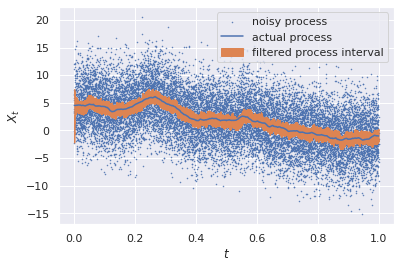
\includegraphics[width=\textwidth]{./resources/Gauss_filter.png}
        \caption{Фильтрация процесса с гауссовским шумом.}
        \label{subfig:Gauss_filter}
    \end{subfigure}
    \hfill
    \begin{subfigure}[b]{0.49\textwidth}
        \centering
        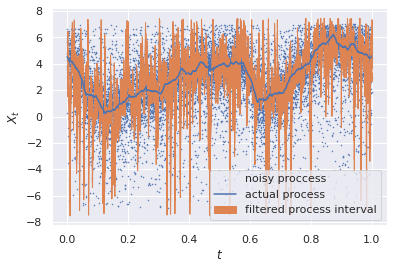
\includegraphics[width=\textwidth]{./resources/Cauchy_filter.png}
        \caption{Фильтрация процесса с шумом распределнным по Коши.}
        \label{subfig:Cauchy_filter}
    \end{subfigure}
    \caption{Фильтрация процесса Орнштейна-Уленбека.}
    \label{fig:filter}
\end{figure}